% Options for packages loaded elsewhere
\PassOptionsToPackage{unicode}{hyperref}
\PassOptionsToPackage{hyphens}{url}
\PassOptionsToPackage{dvipsnames,svgnames,x11names}{xcolor}
%
\documentclass[
  letterpaper,
  DIV=11,
  numbers=noendperiod]{scrartcl}

\usepackage{amsmath,amssymb}
\usepackage{iftex}
\ifPDFTeX
  \usepackage[T1]{fontenc}
  \usepackage[utf8]{inputenc}
  \usepackage{textcomp} % provide euro and other symbols
\else % if luatex or xetex
  \usepackage{unicode-math}
  \defaultfontfeatures{Scale=MatchLowercase}
  \defaultfontfeatures[\rmfamily]{Ligatures=TeX,Scale=1}
\fi
\usepackage{lmodern}
\ifPDFTeX\else  
    % xetex/luatex font selection
    \setmainfont[]{IBM Plex Sans}
    \setsansfont[]{IBM Plex Sans}
    \setmonofont[]{JuliaMono}
\fi
% Use upquote if available, for straight quotes in verbatim environments
\IfFileExists{upquote.sty}{\usepackage{upquote}}{}
\IfFileExists{microtype.sty}{% use microtype if available
  \usepackage[]{microtype}
  \UseMicrotypeSet[protrusion]{basicmath} % disable protrusion for tt fonts
}{}
\makeatletter
\@ifundefined{KOMAClassName}{% if non-KOMA class
  \IfFileExists{parskip.sty}{%
    \usepackage{parskip}
  }{% else
    \setlength{\parindent}{0pt}
    \setlength{\parskip}{6pt plus 2pt minus 1pt}}
}{% if KOMA class
  \KOMAoptions{parskip=half}}
\makeatother
\usepackage{xcolor}
\setlength{\emergencystretch}{3em} % prevent overfull lines
\setcounter{secnumdepth}{-\maxdimen} % remove section numbering
% Make \paragraph and \subparagraph free-standing
\makeatletter
\ifx\paragraph\undefined\else
  \let\oldparagraph\paragraph
  \renewcommand{\paragraph}{
    \@ifstar
      \xxxParagraphStar
      \xxxParagraphNoStar
  }
  \newcommand{\xxxParagraphStar}[1]{\oldparagraph*{#1}\mbox{}}
  \newcommand{\xxxParagraphNoStar}[1]{\oldparagraph{#1}\mbox{}}
\fi
\ifx\subparagraph\undefined\else
  \let\oldsubparagraph\subparagraph
  \renewcommand{\subparagraph}{
    \@ifstar
      \xxxSubParagraphStar
      \xxxSubParagraphNoStar
  }
  \newcommand{\xxxSubParagraphStar}[1]{\oldsubparagraph*{#1}\mbox{}}
  \newcommand{\xxxSubParagraphNoStar}[1]{\oldsubparagraph{#1}\mbox{}}
\fi
\makeatother

\usepackage{color}
\usepackage{fancyvrb}
\newcommand{\VerbBar}{|}
\newcommand{\VERB}{\Verb[commandchars=\\\{\}]}
\DefineVerbatimEnvironment{Highlighting}{Verbatim}{commandchars=\\\{\}}
% Add ',fontsize=\small' for more characters per line
\usepackage{framed}
\definecolor{shadecolor}{RGB}{241,243,245}
\newenvironment{Shaded}{\begin{snugshade}}{\end{snugshade}}
\newcommand{\AlertTok}[1]{\textcolor[rgb]{0.68,0.00,0.00}{#1}}
\newcommand{\AnnotationTok}[1]{\textcolor[rgb]{0.37,0.37,0.37}{#1}}
\newcommand{\AttributeTok}[1]{\textcolor[rgb]{0.40,0.45,0.13}{#1}}
\newcommand{\BaseNTok}[1]{\textcolor[rgb]{0.68,0.00,0.00}{#1}}
\newcommand{\BuiltInTok}[1]{\textcolor[rgb]{0.00,0.23,0.31}{#1}}
\newcommand{\CharTok}[1]{\textcolor[rgb]{0.13,0.47,0.30}{#1}}
\newcommand{\CommentTok}[1]{\textcolor[rgb]{0.37,0.37,0.37}{#1}}
\newcommand{\CommentVarTok}[1]{\textcolor[rgb]{0.37,0.37,0.37}{\textit{#1}}}
\newcommand{\ConstantTok}[1]{\textcolor[rgb]{0.56,0.35,0.01}{#1}}
\newcommand{\ControlFlowTok}[1]{\textcolor[rgb]{0.00,0.23,0.31}{\textbf{#1}}}
\newcommand{\DataTypeTok}[1]{\textcolor[rgb]{0.68,0.00,0.00}{#1}}
\newcommand{\DecValTok}[1]{\textcolor[rgb]{0.68,0.00,0.00}{#1}}
\newcommand{\DocumentationTok}[1]{\textcolor[rgb]{0.37,0.37,0.37}{\textit{#1}}}
\newcommand{\ErrorTok}[1]{\textcolor[rgb]{0.68,0.00,0.00}{#1}}
\newcommand{\ExtensionTok}[1]{\textcolor[rgb]{0.00,0.23,0.31}{#1}}
\newcommand{\FloatTok}[1]{\textcolor[rgb]{0.68,0.00,0.00}{#1}}
\newcommand{\FunctionTok}[1]{\textcolor[rgb]{0.28,0.35,0.67}{#1}}
\newcommand{\ImportTok}[1]{\textcolor[rgb]{0.00,0.46,0.62}{#1}}
\newcommand{\InformationTok}[1]{\textcolor[rgb]{0.37,0.37,0.37}{#1}}
\newcommand{\KeywordTok}[1]{\textcolor[rgb]{0.00,0.23,0.31}{\textbf{#1}}}
\newcommand{\NormalTok}[1]{\textcolor[rgb]{0.00,0.23,0.31}{#1}}
\newcommand{\OperatorTok}[1]{\textcolor[rgb]{0.37,0.37,0.37}{#1}}
\newcommand{\OtherTok}[1]{\textcolor[rgb]{0.00,0.23,0.31}{#1}}
\newcommand{\PreprocessorTok}[1]{\textcolor[rgb]{0.68,0.00,0.00}{#1}}
\newcommand{\RegionMarkerTok}[1]{\textcolor[rgb]{0.00,0.23,0.31}{#1}}
\newcommand{\SpecialCharTok}[1]{\textcolor[rgb]{0.37,0.37,0.37}{#1}}
\newcommand{\SpecialStringTok}[1]{\textcolor[rgb]{0.13,0.47,0.30}{#1}}
\newcommand{\StringTok}[1]{\textcolor[rgb]{0.13,0.47,0.30}{#1}}
\newcommand{\VariableTok}[1]{\textcolor[rgb]{0.07,0.07,0.07}{#1}}
\newcommand{\VerbatimStringTok}[1]{\textcolor[rgb]{0.13,0.47,0.30}{#1}}
\newcommand{\WarningTok}[1]{\textcolor[rgb]{0.37,0.37,0.37}{\textit{#1}}}

\providecommand{\tightlist}{%
  \setlength{\itemsep}{0pt}\setlength{\parskip}{0pt}}\usepackage{longtable,booktabs,array}
\usepackage{calc} % for calculating minipage widths
% Correct order of tables after \paragraph or \subparagraph
\usepackage{etoolbox}
\makeatletter
\patchcmd\longtable{\par}{\if@noskipsec\mbox{}\fi\par}{}{}
\makeatother
% Allow footnotes in longtable head/foot
\IfFileExists{footnotehyper.sty}{\usepackage{footnotehyper}}{\usepackage{footnote}}
\makesavenoteenv{longtable}
\usepackage{graphicx}
\makeatletter
\newsavebox\pandoc@box
\newcommand*\pandocbounded[1]{% scales image to fit in text height/width
  \sbox\pandoc@box{#1}%
  \Gscale@div\@tempa{\textheight}{\dimexpr\ht\pandoc@box+\dp\pandoc@box\relax}%
  \Gscale@div\@tempb{\linewidth}{\wd\pandoc@box}%
  \ifdim\@tempb\p@<\@tempa\p@\let\@tempa\@tempb\fi% select the smaller of both
  \ifdim\@tempa\p@<\p@\scalebox{\@tempa}{\usebox\pandoc@box}%
  \else\usebox{\pandoc@box}%
  \fi%
}
% Set default figure placement to htbp
\def\fps@figure{htbp}
\makeatother

\usepackage{fvextra}
\DefineVerbatimEnvironment{Highlighting}{Verbatim}{breaklines,commandchars=\\\{\}}
\KOMAoption{captions}{tableheading}
\makeatletter
\@ifpackageloaded{caption}{}{\usepackage{caption}}
\AtBeginDocument{%
\ifdefined\contentsname
  \renewcommand*\contentsname{Table of contents}
\else
  \newcommand\contentsname{Table of contents}
\fi
\ifdefined\listfigurename
  \renewcommand*\listfigurename{List of Figures}
\else
  \newcommand\listfigurename{List of Figures}
\fi
\ifdefined\listtablename
  \renewcommand*\listtablename{List of Tables}
\else
  \newcommand\listtablename{List of Tables}
\fi
\ifdefined\figurename
  \renewcommand*\figurename{Figure}
\else
  \newcommand\figurename{Figure}
\fi
\ifdefined\tablename
  \renewcommand*\tablename{Table}
\else
  \newcommand\tablename{Table}
\fi
}
\@ifpackageloaded{float}{}{\usepackage{float}}
\floatstyle{ruled}
\@ifundefined{c@chapter}{\newfloat{codelisting}{h}{lop}}{\newfloat{codelisting}{h}{lop}[chapter]}
\floatname{codelisting}{Listing}
\newcommand*\listoflistings{\listof{codelisting}{List of Listings}}
\makeatother
\makeatletter
\makeatother
\makeatletter
\@ifpackageloaded{caption}{}{\usepackage{caption}}
\@ifpackageloaded{subcaption}{}{\usepackage{subcaption}}
\makeatother

\usepackage{bookmark}

\IfFileExists{xurl.sty}{\usepackage{xurl}}{} % add URL line breaks if available
\urlstyle{same} % disable monospaced font for URLs
\hypersetup{
  pdftitle={Homework 4 Solutions},
  colorlinks=true,
  linkcolor={blue},
  filecolor={Maroon},
  citecolor={Blue},
  urlcolor={Blue},
  pdfcreator={LaTeX via pandoc}}


\title{Homework 4 Solutions}
\usepackage{etoolbox}
\makeatletter
\providecommand{\subtitle}[1]{% add subtitle to \maketitle
  \apptocmd{\@title}{\par {\large #1 \par}}{}{}
}
\makeatother
\subtitle{BEE 4850/5850}
\author{}
\date{}

\begin{document}
\maketitle

\RecustomVerbatimEnvironment{verbatim}{Verbatim}{
showspaces = false,
showtabs = false,
breaksymbolleft={},
breaklines
% Note: setting commandchars=\\\{\} here will cause an error
}


\subsection{Overview}\label{overview}

\subsubsection{Instructions}\label{instructions}

The goal of this homework assignment is to practice simulation-based
uncertainty quantification, including the bootstrap and Markov chain
Monte Carlo.

\begin{itemize}
\tightlist
\item
  Problem 1 asks you to use the parametric and non-parametric bootstrap
  to estimate the median of water level data.
\item
  Problem 2 asks you to use the parametric bootstrap to estimate
  parameter uncertainty in a semi-empirical sea-level rise model.
\item
  Problem 3 (only required for students in BEE 5850) asks you to use the
  bootstrap to quantify uncertainties in the
  gender-impact-on-hurricane-damages dataset from Homework 2.
\end{itemize}

\subsubsection{Load Environment}\label{load-environment}

The following code loads the environment and makes sure all needed
packages are installed. This should be at the start of most Julia
scripts.

\begin{Shaded}
\begin{Highlighting}[]
\ImportTok{import} \BuiltInTok{Pkg}
\BuiltInTok{Pkg}\NormalTok{.}\FunctionTok{activate}\NormalTok{(}\PreprocessorTok{@\_\_DIR\_\_}\NormalTok{)}
\BuiltInTok{Pkg}\NormalTok{.}\FunctionTok{instantiate}\NormalTok{()}
\end{Highlighting}
\end{Shaded}

The following packages are included in the environment (to help you find
other similar packages in other languages). The code below loads these
packages for use in the subsequent notebook (the desired functionality
for each package is commented next to the package).

\begin{Shaded}
\begin{Highlighting}[]
\ImportTok{using} \BuiltInTok{Random} \CommentTok{\# random number generation and seed{-}setting}
\ImportTok{using} \BuiltInTok{DataFrames} \CommentTok{\# tabular data structure}
\ImportTok{using} \BuiltInTok{DataFramesMeta} \CommentTok{\# API which can simplify chains of DataFrames transformations}
\ImportTok{using} \BuiltInTok{CSV\#}\NormalTok{ reads/writes .csv files}
\ImportTok{using} \BuiltInTok{Distributions} \CommentTok{\# interface to work with probability distributions}
\ImportTok{using} \BuiltInTok{Plots} \CommentTok{\# plotting library}
\ImportTok{using} \BuiltInTok{StatsBase} \CommentTok{\# statistical quantities like mean, median, etc}
\ImportTok{using} \BuiltInTok{StatsPlots} \CommentTok{\# some additional statistical plotting tools}
\ImportTok{using} \BuiltInTok{Optim}
\ImportTok{using} \BuiltInTok{LaTeXStrings}
\ImportTok{using} \BuiltInTok{Dates}

\BuiltInTok{Random}\NormalTok{.}\FunctionTok{seed!}\NormalTok{(}\FloatTok{1}\NormalTok{)}
\end{Highlighting}
\end{Shaded}

\subsection{Problems}\label{problems}

\subsubsection{Scoring}\label{scoring}

\begin{itemize}
\tightlist
\item
  Problem 1 is worth 10 points;
\item
  Problem 2 is worth 10 points;
\item
  Problem 3 is worth 5 points.
\end{itemize}

\subsubsection{Problem 1}\label{problem-1}

Let's load the data from `data/salamanders.csv'.

\begin{Shaded}
\begin{Highlighting}[]
\NormalTok{dat }\OperatorTok{=}\NormalTok{ CSV.}\FunctionTok{read}\NormalTok{(}\FunctionTok{joinpath}\NormalTok{(}\StringTok{"data"}\NormalTok{, }\StringTok{"salamanders.csv"}\NormalTok{), DataFrame, delim}\OperatorTok{=}\StringTok{";"}\NormalTok{)}
\end{Highlighting}
\end{Shaded}

\begin{tabular}{r|cccc}
    & SITE & SALAMAN & PCTCOVER & FORESTAGE\\
    \hline
    & Int64 & Int64 & Int64 & Int64\\
    \hline
    1 & 1 & 13 & 85 & 316 \\
    2 & 2 & 11 & 86 & 88 \\
    3 & 3 & 11 & 90 & 548 \\
    4 & 4 & 9 & 88 & 64 \\
    5 & 5 & 8 & 89 & 43 \\
    6 & 6 & 7 & 83 & 368 \\
    7 & 7 & 6 & 83 & 200 \\
    8 & 8 & 6 & 91 & 71 \\
    9 & 9 & 5 & 88 & 42 \\
    10 & 10 & 5 & 90 & 551 \\
    11 & 11 & 4 & 87 & 675 \\
    12 & 12 & 3 & 83 & 217 \\
    13 & 13 & 3 & 87 & 212 \\
    14 & 14 & 3 & 89 & 398 \\
    15 & 15 & 3 & 92 & 357 \\
    16 & 16 & 3 & 93 & 478 \\
    17 & 17 & 2 & 2 & 5 \\
    18 & 18 & 2 & 87 & 30 \\
    19 & 19 & 2 & 93 & 551 \\
    20 & 20 & 1 & 7 & 3 \\
    21 & 21 & 1 & 16 & 15 \\
    22 & 22 & 1 & 19 & 31 \\
    23 & 23 & 1 & 29 & 10 \\
    24 & 24 & 1 & 34 & 49 \\
    $\dots$ & $\dots$ & $\dots$ & $\dots$ & $\dots$ \\
\end{tabular}

Since we're using a Poisson model, the model specification is

\begin{equation*}
\begin{aligned}
y &\sim \text{Poisson}(\lambda) \\
\log(\lambda) &= a x + b,
\end{aligned}
\end{equation*}

where \(x\) is the percent groundcover of the plot and \(y\) is the
salamander count.

Let's find the maximum likelihood.

\begin{Shaded}
\begin{Highlighting}[]
\KeywordTok{function} \FunctionTok{salamander\_pcover}\NormalTok{(p, counts, pctcover) }
\NormalTok{    a, b }\OperatorTok{=}\NormalTok{ p}
\NormalTok{    λ }\OperatorTok{=} \FunctionTok{exp}\NormalTok{.(a }\OperatorTok{*}\NormalTok{ pctcover }\OperatorTok{.+}\NormalTok{ b)}
\NormalTok{    ll }\OperatorTok{=} \FunctionTok{sum}\NormalTok{(}\FunctionTok{logpdf}\NormalTok{.(}\FunctionTok{Poisson}\NormalTok{.(λ), counts))}
    \ControlFlowTok{return}\NormalTok{ ll}
\KeywordTok{end}

\NormalTok{lb }\OperatorTok{=}\NormalTok{ [}\OperatorTok{{-}}\FloatTok{10.0}\NormalTok{, }\OperatorTok{{-}}\FloatTok{50.0}\NormalTok{]}
\NormalTok{ub }\OperatorTok{=}\NormalTok{ [}\FloatTok{10.0}\NormalTok{, }\FloatTok{50.0}\NormalTok{]}
\NormalTok{p0 }\OperatorTok{=}\NormalTok{ [}\FloatTok{0.0}\NormalTok{, }\FloatTok{0.0}\NormalTok{]}

\CommentTok{\# function to make standardizing the predictor more convenient}
\FunctionTok{stdz}\NormalTok{(x) }\OperatorTok{=}\NormalTok{ (x }\OperatorTok{.{-}} \FunctionTok{mean}\NormalTok{(x)) }\OperatorTok{/} \FunctionTok{std}\NormalTok{(x)}

\NormalTok{result }\OperatorTok{=} \FunctionTok{optimize}\NormalTok{(p }\OperatorTok{{-}\textgreater{}} \FunctionTok{{-}salamander\_pcover}\NormalTok{(p, dat.SALAMAN, }\FunctionTok{stdz}\NormalTok{(dat.PCTCOVER)), lb, ub, p0)}
\NormalTok{θ\_mle }\OperatorTok{=}\NormalTok{ result.minimizer}
\end{Highlighting}
\end{Shaded}

\begin{verbatim}
2-element Vector{Float64}:
 1.1595061318756
 0.42951129115546005
\end{verbatim}

Each bootstrap replicate consists of a new dataset formed by resampling
plot datum, to which we repeat the above analysis to refit the model.

\begin{Shaded}
\begin{Highlighting}[]
\NormalTok{nboot }\OperatorTok{=} \FloatTok{1\_000}
\NormalTok{θ\_boot }\OperatorTok{=} \FunctionTok{zeros}\NormalTok{(nboot, }\FloatTok{2}\NormalTok{) }\CommentTok{\# storage for bootstrap replicates}
\ControlFlowTok{for}\NormalTok{ i }\OperatorTok{=} \FloatTok{1}\OperatorTok{:}\NormalTok{nboot}
\NormalTok{    idx }\OperatorTok{=} \FunctionTok{sample}\NormalTok{(}\FloatTok{1}\OperatorTok{:}\FunctionTok{nrow}\NormalTok{(dat), }\FunctionTok{nrow}\NormalTok{(dat), replace}\OperatorTok{=}\ConstantTok{true}\NormalTok{)}
\NormalTok{    boot\_dat }\OperatorTok{=}\NormalTok{ dat[idx, }\OperatorTok{:}\NormalTok{]}
\NormalTok{    result }\OperatorTok{=} \FunctionTok{optimize}\NormalTok{(p }\OperatorTok{{-}\textgreater{}} \FunctionTok{{-}salamander\_pcover}\NormalTok{(p, boot\_dat.SALAMAN, }\FunctionTok{stdz}\NormalTok{(boot\_dat.PCTCOVER)), lb, ub, p0)}
\NormalTok{    θ\_boot[i, }\OperatorTok{:}\NormalTok{] }\OperatorTok{=}\NormalTok{ result.minimizer}
\ControlFlowTok{end}
\CommentTok{\# show the bootstrap mean}
\NormalTok{θ̂ }\OperatorTok{=} \FunctionTok{mean}\NormalTok{(θ\_boot; dims}\OperatorTok{=}\FloatTok{1}\NormalTok{)}
\PreprocessorTok{@show}\NormalTok{ θ̂;}
\end{Highlighting}
\end{Shaded}

\begin{verbatim}
θ̂ = [1.1794723089593893 0.38099303881850943]
\end{verbatim}

We can now visualize the bootstrapped sampling distributions and compare
to the MLE.

\begin{Shaded}
\begin{Highlighting}[]
\NormalTok{p1 }\OperatorTok{=} \FunctionTok{histogram}\NormalTok{(θ\_boot[}\OperatorTok{:}\NormalTok{, }\FloatTok{1}\NormalTok{], xlabel}\OperatorTok{=}\StringTok{"a"}\NormalTok{, ylabel}\OperatorTok{=}\StringTok{"Count"}\NormalTok{, fillcolor}\OperatorTok{=:}\NormalTok{white, label}\OperatorTok{=}\ConstantTok{false}\NormalTok{)}
\FunctionTok{vline!}\NormalTok{(p1, [θ\_mle[}\FloatTok{1}\NormalTok{]], color}\OperatorTok{=:}\NormalTok{red, lw}\OperatorTok{=}\FloatTok{2}\NormalTok{, label}\OperatorTok{=}\StringTok{"MLE"}\NormalTok{)}
\FunctionTok{vline!}\NormalTok{(p1, [θ̂[}\FloatTok{1}\NormalTok{]], color}\OperatorTok{=:}\NormalTok{purple, lw}\OperatorTok{=}\FloatTok{2}\NormalTok{, label}\OperatorTok{=}\StringTok{"Bootstrap Mean"}\NormalTok{)}
\FunctionTok{plot!}\NormalTok{(p1, size}\OperatorTok{=}\NormalTok{(}\FloatTok{400}\NormalTok{, }\FloatTok{400}\NormalTok{))}

\NormalTok{p2 }\OperatorTok{=} \FunctionTok{histogram}\NormalTok{(θ\_boot[}\OperatorTok{:}\NormalTok{, }\FloatTok{2}\NormalTok{], xlabel}\OperatorTok{=}\StringTok{"b"}\NormalTok{, ylabel}\OperatorTok{=}\StringTok{"Count"}\NormalTok{, fillcolor}\OperatorTok{=:}\NormalTok{white, label}\OperatorTok{=}\ConstantTok{false}\NormalTok{)}
\FunctionTok{vline!}\NormalTok{(p2, [θ\_mle[}\FloatTok{2}\NormalTok{]], color}\OperatorTok{=:}\NormalTok{red, lw}\OperatorTok{=}\FloatTok{2}\NormalTok{, label}\OperatorTok{=}\StringTok{"MLE"}\NormalTok{)}
\FunctionTok{vline!}\NormalTok{(p2, [θ̂[}\FloatTok{2}\NormalTok{]], color}\OperatorTok{=:}\NormalTok{purple, lw}\OperatorTok{=}\FloatTok{2}\NormalTok{, label}\OperatorTok{=}\StringTok{"Bootstrap Mean"}\NormalTok{)}
\FunctionTok{plot!}\NormalTok{(p2, size}\OperatorTok{=}\NormalTok{(}\FloatTok{400}\NormalTok{, }\FloatTok{400}\NormalTok{))}

\FunctionTok{display}\NormalTok{(p1)}
\FunctionTok{display}\NormalTok{(p2)}
\end{Highlighting}
\end{Shaded}

\begin{figure}

\begin{minipage}{0.50\linewidth}

\begin{verbatim}
read: Connection reset by peer
send: Broken pipe
\end{verbatim}

\end{minipage}%
%
\begin{minipage}{0.50\linewidth}

\centering{

\pandocbounded{\includegraphics[keepaspectratio]{hw04_files/mediabag/hw04_files/figure-pdf/fig-p1-boot-output-2.pdf}}

}

\subcaption{\label{fig-p1-boot-1}Bootstrapped estimates of parameter
values for Problem 1. The red line is the MLE for the given parameter
and the purple line is the bootstrap mean.}

\end{minipage}%
\newline
\begin{minipage}{0.50\linewidth}

\centering{

\pandocbounded{\includegraphics[keepaspectratio]{hw04_files/mediabag/hw04_files/figure-pdf/fig-p1-boot-output-3.pdf}}

}

\subcaption{\label{fig-p1-boot-2}}

\end{minipage}%

\end{figure}%

We can see from Figure~\ref{fig-p1-boot} that both of the bootstrapped
distributions are skewed, but that the estimates only have a small bias
(recall that the bootstrap estimate of bias of a statistic \(t\) is
\(\mathbb{E}[\tilde{t}] - \hat{t}\), where \(\hat{t}\) is the MLE and
\(\tilde{t}\) is a bootstrap estimate); \(a\) has a bias of 0.02 and
\(b\) has a bias of -0.05.

To find the 90\% confidence intervals, we use the basic bootstrap
formula
\[\left(\hat{t} - (Q_{\tilde{t}}(1-\alpha/2) - \hat{t}), \hat{t} - (Q_{\tilde{t}}(\alpha/2) - \hat{t})\right),\]
where \(\alpha = 0.1\).

\begin{Shaded}
\begin{Highlighting}[]
\NormalTok{a\_q }\OperatorTok{=} \FunctionTok{quantile}\NormalTok{(θ\_boot[}\OperatorTok{:}\NormalTok{, }\FloatTok{1}\NormalTok{], [}\FloatTok{0.95}\NormalTok{, }\FloatTok{0.05}\NormalTok{])}
\NormalTok{b\_q }\OperatorTok{=} \FunctionTok{quantile}\NormalTok{(θ\_boot[}\OperatorTok{:}\NormalTok{, }\FloatTok{2}\NormalTok{], [}\FloatTok{0.95}\NormalTok{, }\FloatTok{0.05}\NormalTok{])}

\NormalTok{a\_ci }\OperatorTok{=}\NormalTok{ (}\FloatTok{2} \OperatorTok{*}\NormalTok{ θ\_mle[}\FloatTok{1}\NormalTok{] }\OperatorTok{{-}}\NormalTok{ a\_q[}\FloatTok{1}\NormalTok{], }\FloatTok{2} \OperatorTok{*}\NormalTok{ θ\_mle[}\FloatTok{1}\NormalTok{] }\OperatorTok{{-}}\NormalTok{ a\_q[}\FloatTok{2}\NormalTok{]) }
\NormalTok{b\_ci }\OperatorTok{=}\NormalTok{ (}\FloatTok{2} \OperatorTok{*}\NormalTok{ θ\_mle[}\FloatTok{2}\NormalTok{] }\OperatorTok{{-}}\NormalTok{ b\_q[}\FloatTok{1}\NormalTok{], }\FloatTok{2} \OperatorTok{*}\NormalTok{ θ\_mle[}\FloatTok{2}\NormalTok{] }\OperatorTok{{-}}\NormalTok{ b\_q[}\FloatTok{2}\NormalTok{]) }
\PreprocessorTok{@show} \FunctionTok{round}\NormalTok{.(a\_ci, digits}\OperatorTok{=}\FloatTok{2}\NormalTok{);}
\PreprocessorTok{@show} \FunctionTok{round}\NormalTok{.(b\_ci, digits}\OperatorTok{=}\FloatTok{2}\NormalTok{);}
\end{Highlighting}
\end{Shaded}

\begin{verbatim}
round.(a_ci, digits = 2) = (0.72, 1.49)
round.(b_ci, digits = 2) = (0.1, 0.91)
\end{verbatim}

One important note is that your answers might differ a bit from these:
the confidence interval estimates are a bit sensitive to the random
bootstrap replicates with this number of replicates, but the answer
should be roughly similar to this.

\subsubsection{Problem 2}\label{problem-2}

First, load the data

\begin{Shaded}
\begin{Highlighting}[]

\NormalTok{norm\_yrs }\OperatorTok{=} \FloatTok{1980}\OperatorTok{:}\FloatTok{1999}

\NormalTok{sl\_dat }\OperatorTok{=} \FunctionTok{DataFrame}\NormalTok{(CSV.}\FunctionTok{File}\NormalTok{(}\FunctionTok{joinpath}\NormalTok{(}\StringTok{"data"}\NormalTok{,  }\StringTok{"CSIRO\_Recons\_gmsl\_yr\_2015.csv"}\NormalTok{)))}

\FunctionTok{rename!}\NormalTok{(sl\_dat, [}\OperatorTok{:}\NormalTok{Year, }\OperatorTok{:}\NormalTok{GMSLR, }\OperatorTok{:}\NormalTok{SD]) }\CommentTok{\# rename to make columns easier to work with}
\NormalTok{sl\_dat[!, }\OperatorTok{:}\NormalTok{Year] }\OperatorTok{.{-}=} \FloatTok{0.5} \CommentTok{\# shift year to line up with years instead of being half{-}year }
\NormalTok{sl\_dat[!, }\OperatorTok{:}\NormalTok{GMSLR] }\OperatorTok{.{-}=} \FunctionTok{mean}\NormalTok{(}\FunctionTok{filter}\NormalTok{(row }\OperatorTok{{-}\textgreater{}}\NormalTok{ row.Year }\OperatorTok{∈}\NormalTok{ norm\_yrs, sl\_dat)[!, }\OperatorTok{:}\NormalTok{GMSLR]) }\CommentTok{\# rescale to be relative to 1880{-}1900 mean for consistency with temperature anomaly}

\CommentTok{\# load temperature data}
\NormalTok{temp\_dat }\OperatorTok{=} \FunctionTok{DataFrame}\NormalTok{(CSV.}\FunctionTok{File}\NormalTok{(}\FunctionTok{joinpath}\NormalTok{(}\StringTok{"data"}\NormalTok{, }\StringTok{"HadCRUT.5.0.2.0.analysis.summary\_series.global.annual.csv"}\NormalTok{)))}
\FunctionTok{rename!}\NormalTok{(temp\_dat, [}\OperatorTok{:}\NormalTok{Year, }\OperatorTok{:}\NormalTok{Temp, }\OperatorTok{:}\NormalTok{Lower, }\OperatorTok{:}\NormalTok{Upper]) }\CommentTok{\# rename to make columns easier to work with}
\FunctionTok{filter!}\NormalTok{(row }\OperatorTok{{-}\textgreater{}}\NormalTok{ row.Year }\OperatorTok{∈}\NormalTok{ sl\_dat[!, }\OperatorTok{:}\NormalTok{Year], temp\_dat) }\CommentTok{\# reduce to the same years that we have SL data for}
\NormalTok{temp\_normalize }\OperatorTok{=} \FunctionTok{mean}\NormalTok{(}\FunctionTok{filter}\NormalTok{(row }\OperatorTok{{-}\textgreater{}}\NormalTok{ row.Year }\OperatorTok{∈}\NormalTok{ norm\_yrs, temp\_dat)[!, }\OperatorTok{:}\NormalTok{Temp]) }\CommentTok{\# get renormalization to rescale temperature to 1880{-}1900 mean}
\NormalTok{temp\_dat[!, }\OperatorTok{:}\NormalTok{Temp] }\OperatorTok{.{-}=}\NormalTok{ temp\_normalize}
\NormalTok{temp\_dat[!, }\OperatorTok{:}\NormalTok{Lower] }\OperatorTok{.{-}=}\NormalTok{ temp\_normalize}
\NormalTok{temp\_dat[!, }\OperatorTok{:}\NormalTok{Upper] }\OperatorTok{.{-}=}\NormalTok{  temp\_normalize}

\NormalTok{sl\_plot }\OperatorTok{=} \FunctionTok{scatter}\NormalTok{(sl\_dat[!, }\OperatorTok{:}\NormalTok{Year], sl\_dat[!, }\OperatorTok{:}\NormalTok{GMSLR], yerr}\OperatorTok{=}\NormalTok{sl\_dat[!, }\OperatorTok{:}\NormalTok{SD], color}\OperatorTok{=:}\NormalTok{black, label}\OperatorTok{=}\StringTok{"Observations"}\NormalTok{, ylabel}\OperatorTok{=}\StringTok{"(mm)"}\NormalTok{, xlabel}\OperatorTok{=}\StringTok{"Year"}\NormalTok{, title}\OperatorTok{=}\StringTok{"Sea Level Anomaly"}\NormalTok{)}

\NormalTok{temp\_plot }\OperatorTok{=} \FunctionTok{scatter}\NormalTok{(temp\_dat[!, }\OperatorTok{:}\NormalTok{Year], temp\_dat[!, }\OperatorTok{:}\NormalTok{Temp], yerr}\OperatorTok{=}\NormalTok{(temp\_dat[!, }\OperatorTok{:}\NormalTok{Temp] }\OperatorTok{{-}}\NormalTok{ temp\_dat[!, }\OperatorTok{:}\NormalTok{Lower], temp\_dat[!, }\OperatorTok{:}\NormalTok{Upper] }\OperatorTok{{-}}\NormalTok{ temp\_dat[!, }\OperatorTok{:}\NormalTok{Temp]), color}\OperatorTok{=:}\NormalTok{black, label}\OperatorTok{=}\StringTok{"Observations"}\NormalTok{, ylabel}\OperatorTok{=}\StringTok{"(°C)"}\NormalTok{, xlabel}\OperatorTok{=}\StringTok{"Year"}\NormalTok{, title}\OperatorTok{=}\StringTok{"Temperature"}\NormalTok{)}
\end{Highlighting}
\end{Shaded}

\pandocbounded{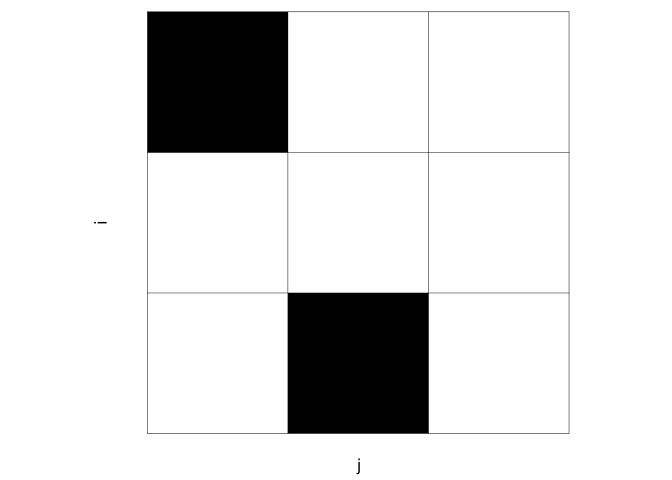
\includegraphics[keepaspectratio]{hw04_files/mediabag/hw04_files/figure-pdf/cell-9-output-1.pdf}}

The Grinsted model in code (skipping past the discretization since we
did this in HW2):

\begin{Shaded}
\begin{Highlighting}[]
\KeywordTok{function} \FunctionTok{grinsted\_slr}\NormalTok{(params, temps; Δt}\OperatorTok{=}\FloatTok{1}\NormalTok{)}
\NormalTok{    a, b, τ, S₀ }\OperatorTok{=}\NormalTok{ params}
\NormalTok{    S }\OperatorTok{=} \FunctionTok{zeros}\NormalTok{(}\FunctionTok{length}\NormalTok{(temps)) }\CommentTok{\# initialize storage}
\NormalTok{    Seq }\OperatorTok{=}\NormalTok{ a }\OperatorTok{*}\NormalTok{ temps }\OperatorTok{.+}\NormalTok{ b}
\NormalTok{    S[}\FloatTok{1}\NormalTok{] }\OperatorTok{=}\NormalTok{ S₀}
    \ControlFlowTok{for}\NormalTok{ i }\OperatorTok{=} \FloatTok{2}\OperatorTok{:}\FunctionTok{length}\NormalTok{(S)}
\NormalTok{        S[i] }\OperatorTok{=}\NormalTok{ S[i}\OperatorTok{{-}}\FloatTok{1}\NormalTok{] }\OperatorTok{+}\NormalTok{  Δt }\OperatorTok{*}\NormalTok{ (Seq[i] }\OperatorTok{{-}}\NormalTok{ S[i}\OperatorTok{{-}}\FloatTok{1}\NormalTok{]) }\OperatorTok{/}\NormalTok{ τ}
    \ControlFlowTok{end}
    \ControlFlowTok{return}\NormalTok{ S[}\FloatTok{1}\OperatorTok{:}\KeywordTok{end}\NormalTok{]}
\KeywordTok{end}
\end{Highlighting}
\end{Shaded}

\begin{verbatim}
grinsted_slr (generic function with 1 method)
\end{verbatim}

The log likelihood function with AR(1) residuals:

\begin{Shaded}
\begin{Highlighting}[]
\KeywordTok{function} \FunctionTok{ar1\_loglik}\NormalTok{(params, temp\_dat, slr\_obs, Δt}\OperatorTok{=}\FloatTok{1.0}\NormalTok{)}
\NormalTok{    a, b, τ, S₀, ρ, σ }\OperatorTok{=}\NormalTok{ params }
\NormalTok{    slr\_sim }\OperatorTok{=} \FunctionTok{grinsted\_slr}\NormalTok{((a, b, τ, S₀), temp\_dat; Δt }\OperatorTok{=}\NormalTok{ Δt)}
    \CommentTok{\# whiten residuals}
\NormalTok{    resids }\OperatorTok{=}\NormalTok{ slr\_obs }\OperatorTok{.{-}}\NormalTok{ slr\_sim}
\NormalTok{    ll }\OperatorTok{=} \FloatTok{0}
    \ControlFlowTok{for}\NormalTok{ t }\OperatorTok{=} \FloatTok{1}\OperatorTok{:}\FunctionTok{length}\NormalTok{(temp\_dat) }\OperatorTok{{-}} \FloatTok{1}
        \ControlFlowTok{if}\NormalTok{ t }\OperatorTok{==} \FloatTok{1}
\NormalTok{            ll }\OperatorTok{+=} \FunctionTok{logpdf}\NormalTok{(}\FunctionTok{Normal}\NormalTok{(}\FloatTok{0}\NormalTok{, }\FunctionTok{sqrt}\NormalTok{(σ}\OperatorTok{\^{}}\FloatTok{2} \OperatorTok{/}\NormalTok{ (}\FloatTok{1} \OperatorTok{{-}}\NormalTok{ ρ}\OperatorTok{\^{}}\FloatTok{2}\NormalTok{))), resids[t])}
        \ControlFlowTok{else}
\NormalTok{            ll }\OperatorTok{+=} \FunctionTok{sum}\NormalTok{(}\FunctionTok{logpdf}\NormalTok{(}\FunctionTok{Normal}\NormalTok{(ρ }\OperatorTok{*}\NormalTok{ resids[t], σ), resids[t}\OperatorTok{+}\FloatTok{1}\NormalTok{]))}
        \ControlFlowTok{end}
    \ControlFlowTok{end} 
    \ControlFlowTok{return}\NormalTok{ ll}
\KeywordTok{end}
\end{Highlighting}
\end{Shaded}

\begin{verbatim}
ar1_loglik (generic function with 2 methods)
\end{verbatim}

Now, let's find the MLE by optimizing the \texttt{ar1\_loglik} function.

\begin{Shaded}
\begin{Highlighting}[]
\NormalTok{low\_bds }\OperatorTok{=}\NormalTok{ [}\OperatorTok{{-}}\FloatTok{2000.0}\NormalTok{, }\OperatorTok{{-}}\FloatTok{2000.0}\NormalTok{, }\FloatTok{0.1}\NormalTok{, sl\_dat.GMSLR[}\FloatTok{1}\NormalTok{] }\OperatorTok{{-}} \FloatTok{1.96} \OperatorTok{*}\NormalTok{ sl\_dat.SD[}\FloatTok{1}\NormalTok{], }\OperatorTok{{-}}\FloatTok{1.0}\NormalTok{, }\FloatTok{0.1}\NormalTok{]}
\NormalTok{up\_bds }\OperatorTok{=}\NormalTok{ [}\FloatTok{20\_000.0}\NormalTok{, }\FloatTok{30\_000.0}\NormalTok{, }\FloatTok{10\_000.0}\NormalTok{, sl\_dat.GMSLR[}\FloatTok{1}\NormalTok{] }\OperatorTok{+} \FloatTok{1.96} \OperatorTok{*}\NormalTok{ sl\_dat.SD[}\FloatTok{1}\NormalTok{], }\FloatTok{0.99}\NormalTok{, }\FloatTok{100.0}\NormalTok{]}
\NormalTok{p₀ }\OperatorTok{=}\NormalTok{ [}\FloatTok{10.0}\NormalTok{, }\FloatTok{0.0}\NormalTok{, }\FloatTok{1500.0}\NormalTok{, sl\_dat.GMSLR[}\FloatTok{1}\NormalTok{], }\FloatTok{0.0}\NormalTok{, }\FloatTok{10.0}\NormalTok{]}

\NormalTok{mle\_optim }\OperatorTok{=} \FunctionTok{optimize}\NormalTok{(p }\OperatorTok{{-}\textgreater{}} \FunctionTok{{-}ar1\_loglik}\NormalTok{(p, temp\_dat.Temp, sl\_dat.GMSLR), low\_bds, up\_bds, p₀)}
\NormalTok{p\_mle }\OperatorTok{=}\NormalTok{ mle\_optim.minimizer}
\PreprocessorTok{@show}\NormalTok{ p\_mle;}
\end{Highlighting}
\end{Shaded}

\begin{verbatim}
p_mle = [546.9549427127922, 410.3873816251446, 179.69518456677608, -158.18775262248883, 0.5215568507538185, 4.960943964640367]
\end{verbatim}

We can plot the fitted model and the residuals:

\begin{Shaded}
\begin{Highlighting}[]
\NormalTok{slr\_fit }\OperatorTok{=} \FunctionTok{grinsted\_slr}\NormalTok{(p\_mle[}\FloatTok{1}\OperatorTok{:}\KeywordTok{end}\OperatorTok{{-}}\FloatTok{2}\NormalTok{], temp\_dat.Temp)}
\NormalTok{resids }\OperatorTok{=}\NormalTok{ sl\_dat.GMSLR }\OperatorTok{{-}}\NormalTok{ slr\_fit}

\NormalTok{pfit }\OperatorTok{=} \FunctionTok{plot}\NormalTok{(sl\_dat.Year, slr\_fit, color}\OperatorTok{=:}\NormalTok{blue, xlabel}\OperatorTok{=}\StringTok{"Year"}\NormalTok{, ylabel}\OperatorTok{=}\StringTok{"Global Mean Sea Level (mm)"}\NormalTok{, label}\OperatorTok{=}\StringTok{"Model Fit"}\NormalTok{)}
\FunctionTok{scatter!}\NormalTok{(pfit, sl\_dat.Year, sl\_dat.GMSLR, color}\OperatorTok{=:}\NormalTok{black, label}\OperatorTok{=}\StringTok{"Observations"}\NormalTok{)}
\FunctionTok{plot!}\NormalTok{(pfit, size}\OperatorTok{=}\NormalTok{(}\FloatTok{400}\NormalTok{, }\FloatTok{400}\NormalTok{))}

\NormalTok{presids }\OperatorTok{=} \FunctionTok{scatter}\NormalTok{(sl\_dat.Year, resids, color}\OperatorTok{=:}\NormalTok{black, xlabel}\OperatorTok{=}\StringTok{"Year"}\NormalTok{, ylabel}\OperatorTok{=}\StringTok{"Model Residuals (mm)"}\NormalTok{, legend}\OperatorTok{=}\ConstantTok{false}\NormalTok{)}
\FunctionTok{plot!}\NormalTok{(presids, size}\OperatorTok{=}\NormalTok{(}\FloatTok{400}\NormalTok{, }\FloatTok{400}\NormalTok{))}

\FunctionTok{display}\NormalTok{(pfit)}
\FunctionTok{display}\NormalTok{(presids)}
\end{Highlighting}
\end{Shaded}

\begin{figure}

\begin{minipage}{0.50\linewidth}

\begin{verbatim}
read: Connection reset by peer
send: Broken pipe
\end{verbatim}

\end{minipage}%
%
\begin{minipage}{0.50\linewidth}

\centering{

\pandocbounded{\includegraphics[keepaspectratio]{hw04_files/mediabag/hw04_files/figure-pdf/fig-p2-fit-output-2.pdf}}

}

\subcaption{\label{fig-p2-fit-1}Sea-level hindcast using the fitted
Grinsted model and the model residuals.}

\end{minipage}%
\newline
\begin{minipage}{0.50\linewidth}

\centering{

\pandocbounded{\includegraphics[keepaspectratio]{hw04_files/mediabag/hw04_files/figure-pdf/fig-p2-fit-output-3.pdf}}

}

\subcaption{\label{fig-p2-fit-2}}

\end{minipage}%

\end{figure}%

Now we want to generate 1,000 replicates of the residuals using the
fitted AR(1) process and add them back to the model hindcast.

\begin{Shaded}
\begin{Highlighting}[]
\KeywordTok{function} \FunctionTok{ar1\_sim}\NormalTok{(ρ, σ, n\_sim, T)}

\NormalTok{    sim\_out }\OperatorTok{=} \FunctionTok{zeros}\NormalTok{(n\_sim, T)}
    \ControlFlowTok{for}\NormalTok{ t }\OperatorTok{=} \FloatTok{1}\OperatorTok{:}\NormalTok{T}
        \ControlFlowTok{if}\NormalTok{ t }\OperatorTok{==} \FloatTok{1}
\NormalTok{            sim\_out[}\OperatorTok{:}\NormalTok{, t] }\OperatorTok{=} \FunctionTok{rand}\NormalTok{(}\FunctionTok{Normal}\NormalTok{(}\FloatTok{0}\NormalTok{, }\FunctionTok{sqrt}\NormalTok{(σ}\OperatorTok{\^{}}\FloatTok{2} \OperatorTok{/}\NormalTok{ (}\FloatTok{1} \OperatorTok{{-}}\NormalTok{ ρ}\OperatorTok{\^{}}\FloatTok{2}\NormalTok{))), n\_sim)}
        \ControlFlowTok{else}
\NormalTok{            sim\_out[}\OperatorTok{:}\NormalTok{, t] }\OperatorTok{=} \FunctionTok{rand}\NormalTok{.(}\FunctionTok{Normal}\NormalTok{.(ρ }\OperatorTok{*}\NormalTok{ sim\_out[}\OperatorTok{:}\NormalTok{, t}\OperatorTok{{-}}\FloatTok{1}\NormalTok{], σ))}
        \ControlFlowTok{end}
    \ControlFlowTok{end}
    \ControlFlowTok{return}\NormalTok{ sim\_out}
\KeywordTok{end}

\NormalTok{n\_sim }\OperatorTok{=} \FloatTok{1\_000}
\NormalTok{resids\_boot }\OperatorTok{=} \FunctionTok{ar1\_sim}\NormalTok{(p\_mle[}\KeywordTok{end}\OperatorTok{{-}}\FloatTok{1}\NormalTok{], p\_mle[}\KeywordTok{end}\NormalTok{], n\_sim, }\FunctionTok{nrow}\NormalTok{(temp\_dat))}
\NormalTok{slr\_boot }\OperatorTok{=} \FunctionTok{mapslices}\NormalTok{(row }\OperatorTok{{-}\textgreater{}}\NormalTok{ row }\OperatorTok{.+}\NormalTok{ slr\_fit, resids\_boot; dims}\OperatorTok{=}\FloatTok{2}\NormalTok{)}
\end{Highlighting}
\end{Shaded}

\begin{verbatim}
1000×134 Matrix{Float64}:
 -155.578  -160.371  -150.263  …  65.6277  66.8024  60.9281  66.3092
 -166.817  -150.491  -144.177     50.7711  53.8146  58.418   54.321
 -159.91   -162.683  -163.252     50.7926  68.1767  61.0413  63.3705
 -162.234  -151.419  -150.336     56.3515  66.5042  65.2169  70.7606
 -154.785  -153.74   -152.474     53.0952  59.1195  62.5341  61.0469
 -158.985  -157.702  -154.061  …  53.8543  58.2929  60.5728  58.7454
 -161.992  -149.346  -157.096     57.0526  65.5743  61.8247  55.8163
 -157.933  -162.833  -164.287     52.874   55.6301  63.7023  70.2268
 -157.496  -149.485  -152.446     48.1722  47.95    52.4044  63.0504
 -145.989  -149.469  -149.711     64.1377  57.1585  53.9137  51.6984
    ⋮                          ⋱   ⋮                         
 -152.459  -161.553  -158.747     61.4694  70.3682  68.5933  74.4939
 -163.098  -154.776  -146.78      59.051   64.7032  62.6031  66.4458
 -156.917  -158.073  -143.377     64.4128  63.236   70.6126  71.2534
 -158.449  -159.636  -159.65      62.12    60.2227  61.7398  67.2607
 -151.149  -152.926  -151.828  …  55.7968  62.4473  62.726   64.2052
 -159.789  -161.955  -157.092     63.7249  59.6974  61.7888  64.13
 -159.274  -154.538  -146.59      54.7705  62.0086  53.6441  63.3536
 -164.655  -157.275  -162.345     46.6267  49.4417  59.9164  62.2635
 -151.977  -153.05   -153.809     50.9142  62.5265  58.7918  65.9182
\end{verbatim}

Now we refit the model to each replicate to get the estimates of the
bootstrap parameters.

\begin{Shaded}
\begin{Highlighting}[]
\NormalTok{a\_boot }\OperatorTok{=} \FunctionTok{zeros}\NormalTok{(n\_sim)}
\NormalTok{b\_boot }\OperatorTok{=} \FunctionTok{zeros}\NormalTok{(n\_sim)}
\NormalTok{τ\_boot }\OperatorTok{=} \FunctionTok{zeros}\NormalTok{(n\_sim)}
\NormalTok{S₀\_boot }\OperatorTok{=} \FunctionTok{zeros}\NormalTok{(n\_sim)}
\NormalTok{ρ\_boot }\OperatorTok{=} \FunctionTok{zeros}\NormalTok{(n\_sim)}
\NormalTok{σ\_boot }\OperatorTok{=} \FunctionTok{zeros}\NormalTok{(n\_sim)}

\ControlFlowTok{for}\NormalTok{ i }\OperatorTok{=} \FloatTok{1}\OperatorTok{:}\NormalTok{n\_sim}
\NormalTok{    mle\_optim }\OperatorTok{=} \FunctionTok{optimize}\NormalTok{(p }\OperatorTok{{-}\textgreater{}} \FunctionTok{{-}ar1\_loglik}\NormalTok{(p, temp\_dat.Temp, slr\_boot[i, }\OperatorTok{:}\NormalTok{]), low\_bds, up\_bds, p₀)}
\NormalTok{    a\_boot[i], b\_boot[i], τ\_boot[i], S₀\_boot[i], ρ\_boot[i], σ\_boot[i] }\OperatorTok{=}\NormalTok{ mle\_optim.minimizer}
\ControlFlowTok{end}
\end{Highlighting}
\end{Shaded}

Plotting the histograms:

\begin{Shaded}
\begin{Highlighting}[]
\NormalTok{hist1 }\OperatorTok{=} \FunctionTok{histogram}\NormalTok{(a\_boot, xlabel}\OperatorTok{=}\NormalTok{L}\StringTok{"}\SpecialCharTok{$}\NormalTok{a}\SpecialCharTok{$}\StringTok{", }\NormalTok{ylabel}\StringTok{="}\NormalTok{Count}\StringTok{", legend=false, title=L"}\OperatorTok{$}\NormalTok{a}\OperatorTok{$}\StringTok{")}
\FunctionTok{vline!}\NormalTok{(hist1, [p\_mle[}\FloatTok{1}\NormalTok{]], color}\OperatorTok{=:}\NormalTok{red)}
\FunctionTok{plot!}\NormalTok{(hist1, size}\OperatorTok{=}\NormalTok{(}\FloatTok{300}\NormalTok{, }\FloatTok{300}\NormalTok{))}

\NormalTok{hist2 }\OperatorTok{=} \FunctionTok{histogram}\NormalTok{(b\_boot, xlabel}\OperatorTok{=}\NormalTok{L}\StringTok{"}\SpecialCharTok{$}\NormalTok{b}\SpecialCharTok{$}\StringTok{", }\NormalTok{ylabel}\StringTok{="}\NormalTok{Count}\StringTok{", legend=false, title=L"}\OperatorTok{$}\NormalTok{b}\OperatorTok{$}\StringTok{")}
\FunctionTok{vline!}\NormalTok{(hist2, [p\_mle[}\FloatTok{2}\NormalTok{]], color}\OperatorTok{=:}\NormalTok{red)}
\FunctionTok{plot!}\NormalTok{(hist2, size}\OperatorTok{=}\NormalTok{(}\FloatTok{300}\NormalTok{, }\FloatTok{300}\NormalTok{))}

\NormalTok{hist3 }\OperatorTok{=} \FunctionTok{histogram}\NormalTok{(τ\_boot, xlabel}\OperatorTok{=}\NormalTok{L}\StringTok{"}\SpecialCharTok{$}\StringTok{\textbackslash{}}\NormalTok{tau}\SpecialCharTok{$}\StringTok{", }\NormalTok{ylabel}\StringTok{="}\NormalTok{Count}\StringTok{", legend=false, title=L"}\OperatorTok{$\textbackslash{}}\NormalTok{tau}\OperatorTok{$}\StringTok{")}
\FunctionTok{vline!}\NormalTok{(hist3, [p\_mle[}\FloatTok{3}\NormalTok{]], color}\OperatorTok{=:}\NormalTok{red)}
\FunctionTok{plot!}\NormalTok{(hist3, size}\OperatorTok{=}\NormalTok{(}\FloatTok{300}\NormalTok{, }\FloatTok{300}\NormalTok{))}

\NormalTok{hist4 }\OperatorTok{=} \FunctionTok{histogram}\NormalTok{(S₀\_boot, xlabel}\OperatorTok{=}\NormalTok{L}\StringTok{"}\SpecialCharTok{$}\NormalTok{S\_0}\SpecialCharTok{$}\StringTok{", }\NormalTok{ylabel}\StringTok{="}\NormalTok{Count}\StringTok{", legend=false, title=L"}\OperatorTok{$}\NormalTok{S\_0}\OperatorTok{$}\StringTok{")}
\FunctionTok{vline!}\NormalTok{(hist4, [p\_mle[}\FloatTok{4}\NormalTok{]], color}\OperatorTok{=:}\NormalTok{red)}
\FunctionTok{plot!}\NormalTok{(hist4, size}\OperatorTok{=}\NormalTok{(}\FloatTok{300}\NormalTok{, }\FloatTok{300}\NormalTok{))}

\NormalTok{hist5 }\OperatorTok{=} \FunctionTok{histogram}\NormalTok{(ρ\_boot, xlabel}\OperatorTok{=}\NormalTok{L}\StringTok{"}\SpecialCharTok{$}\StringTok{\textbackslash{}}\NormalTok{rho}\SpecialCharTok{$}\StringTok{", }\NormalTok{ylabel}\StringTok{="}\NormalTok{Count}\StringTok{", legend=false, title=L"}\OperatorTok{$\textbackslash{}}\NormalTok{rho}\OperatorTok{$}\StringTok{")}
\FunctionTok{vline!}\NormalTok{(hist5, [p\_mle[}\FloatTok{5}\NormalTok{]], color}\OperatorTok{=:}\NormalTok{red)}
\FunctionTok{plot!}\NormalTok{(hist5, size}\OperatorTok{=}\NormalTok{(}\FloatTok{300}\NormalTok{, }\FloatTok{300}\NormalTok{))}

\NormalTok{hist6 }\OperatorTok{=} \FunctionTok{histogram}\NormalTok{(σ\_boot, xlabel}\OperatorTok{=}\NormalTok{L}\StringTok{"}\SpecialCharTok{$}\StringTok{\textbackslash{}}\NormalTok{sigma}\SpecialCharTok{$}\StringTok{", }\NormalTok{ylabel}\StringTok{="}\NormalTok{Count}\StringTok{", legend=false, title=L"}\OperatorTok{$\textbackslash{}}\NormalTok{sigma}\OperatorTok{$}\StringTok{")}
\FunctionTok{vline!}\NormalTok{(hist6, [p\_mle[}\FloatTok{6}\NormalTok{]], color}\OperatorTok{=:}\NormalTok{red)}
\FunctionTok{plot!}\NormalTok{(hist6, size}\OperatorTok{=}\NormalTok{(}\FloatTok{300}\NormalTok{, }\FloatTok{300}\NormalTok{))}

\FunctionTok{display}\NormalTok{(hist1)}
\FunctionTok{display}\NormalTok{(hist2)}
\FunctionTok{display}\NormalTok{(hist3)}
\FunctionTok{display}\NormalTok{(hist4)}
\FunctionTok{display}\NormalTok{(hist5)}
\FunctionTok{display}\NormalTok{(hist6)}
\end{Highlighting}
\end{Shaded}

\begin{figure}

\begin{minipage}{0.50\linewidth}

\begin{verbatim}
read: Connection reset by peer
send: Broken pipe
read: Connection reset by peer
send: Broken pipe
\end{verbatim}

\end{minipage}%
%
\begin{minipage}{0.50\linewidth}

\centering{

\pandocbounded{\includegraphics[keepaspectratio]{hw04_files/mediabag/hw04_files/figure-pdf/fig-p2-samples-output-2.pdf}}

}

\subcaption{\label{fig-p2-samples-1}Bootstrap samples for each
parameter. The red line is the MLE.}

\end{minipage}%
\newline
\begin{minipage}{0.50\linewidth}

\centering{

\pandocbounded{\includegraphics[keepaspectratio]{hw04_files/mediabag/hw04_files/figure-pdf/fig-p2-samples-output-3.pdf}}

}

\subcaption{\label{fig-p2-samples-2}}

\end{minipage}%
%
\begin{minipage}{0.50\linewidth}

\centering{

\pandocbounded{\includegraphics[keepaspectratio]{hw04_files/mediabag/hw04_files/figure-pdf/fig-p2-samples-output-4.pdf}}

}

\subcaption{\label{fig-p2-samples-3}}

\end{minipage}%
\newline
\begin{minipage}{0.50\linewidth}

\centering{

\pandocbounded{\includegraphics[keepaspectratio]{hw04_files/mediabag/hw04_files/figure-pdf/fig-p2-samples-output-5.pdf}}

}

\subcaption{\label{fig-p2-samples-4}}

\end{minipage}%
%
\begin{minipage}{0.50\linewidth}

\centering{

\pandocbounded{\includegraphics[keepaspectratio]{hw04_files/mediabag/hw04_files/figure-pdf/fig-p2-samples-output-6.pdf}}

}

\subcaption{\label{fig-p2-samples-5}}

\end{minipage}%
\newline
\begin{minipage}{0.50\linewidth}

\centering{

\pandocbounded{\includegraphics[keepaspectratio]{hw04_files/mediabag/hw04_files/figure-pdf/fig-p2-samples-output-7.pdf}}

}

\subcaption{\label{fig-p2-samples-6}}

\end{minipage}%

\end{figure}%

We can see that there are some outlying replicates which result in very
high bootstrap samples for the model parameters \(a\), \(b\), and
\(\tau\). But now we can calculate the sampling distribution of the
sea-level sensitivity to temperature, which is \(a/\tau\). Plotting this
distribution:

\begin{Shaded}
\begin{Highlighting}[]
\NormalTok{sens }\OperatorTok{=}\NormalTok{ a\_boot }\OperatorTok{./}\NormalTok{ τ\_boot}

\NormalTok{psens }\OperatorTok{=} \FunctionTok{histogram}\NormalTok{(sens, xlabel}\OperatorTok{=}\StringTok{"Sea{-}Level Sensitivity to Temperature (mm/°C)"}\NormalTok{, ylabel}\OperatorTok{=}\StringTok{"Count"}\NormalTok{, label}\OperatorTok{=}\ConstantTok{false}\NormalTok{)}
\FunctionTok{vline!}\NormalTok{(psens, [p\_mle[}\FloatTok{1}\NormalTok{] }\OperatorTok{/}\NormalTok{ p\_mle[}\FloatTok{3}\NormalTok{]], color}\OperatorTok{=:}\NormalTok{red, label}\OperatorTok{=}\StringTok{"MLE"}\NormalTok{)}
\FunctionTok{plot!}\NormalTok{(psens, size}\OperatorTok{=}\NormalTok{(}\FloatTok{600}\NormalTok{, }\FloatTok{400}\NormalTok{))}
\end{Highlighting}
\end{Shaded}

\begin{figure}[H]

\centering{

\pandocbounded{\includegraphics[keepaspectratio]{hw04_files/mediabag/hw04_files/figure-pdf/fig-p2-sensitivity-output-1.pdf}}

}

\caption{\label{fig-p2-sensitivity}Bootstrap distribution for the
sea-level sensitivity to temperature. The red line is the MLE.}

\end{figure}%

We can see from Figure~\ref{fig-p2-sensitivity} that the large outlying
samples cancel out in terms of the numerical effect, which is why the
model fit still worked well.\footnote{This also highlights a key point
  for model calibration and statistical inference: individual model
  parameters may not be directly interpretable due to these compensating
  effects, and it's valuable to look at physically-relevant statistics
  rather than specific parameters. If the individual model parameters
  are important for interpretation or extrapolation, they should be
  appropriately constrained or prior information should be used through
  a Bayesian analysis.}

The 90\% basic bootstrap confidence interval then becomes

\begin{Shaded}
\begin{Highlighting}[]
\NormalTok{sens\_mle }\OperatorTok{=}\NormalTok{ p\_mle[}\FloatTok{1}\NormalTok{] }\OperatorTok{/}\NormalTok{ p\_mle[}\FloatTok{3}\NormalTok{]}
\NormalTok{q\_boot }\OperatorTok{=} \FunctionTok{quantile}\NormalTok{(sens, [}\FloatTok{0.95}\NormalTok{, }\FloatTok{0.05}\NormalTok{])}
\NormalTok{ci\_boot }\OperatorTok{=} \FloatTok{2} \OperatorTok{*}\NormalTok{ sens\_mle }\OperatorTok{.{-}}\NormalTok{ q\_boot}
\FunctionTok{vspan!}\NormalTok{(psens, ci\_boot, linecolor}\OperatorTok{=:}\NormalTok{grey, fillcolor}\OperatorTok{=:}\NormalTok{grey, alpha}\OperatorTok{=}\FloatTok{0.3}\NormalTok{, fillalpha}\OperatorTok{=}\FloatTok{0.3}\NormalTok{, label}\OperatorTok{=}\StringTok{"90\% CI"}\NormalTok{)}
\end{Highlighting}
\end{Shaded}

\begin{figure}[H]

\centering{

\pandocbounded{\includegraphics[keepaspectratio]{hw04_files/mediabag/hw04_files/figure-pdf/fig-p2-sensitivity-ci-output-1.pdf}}

}

\caption{\label{fig-p2-sensitivity-ci}Bootstrap distribution for the
sea-level sensitivity to temperature. The red line is the MLE. The grey
region is the 90\% confidence interval estimated using the basic
bootstrap method.}

\end{figure}%

The values for the 90\% CI are {[}1.3, 4.3{]}, and the MLE is 3.0. We
can see the impact of the skewed distribution in
Figure~\ref{fig-p2-sensitivity-ci}.

\subsubsection{Problem 3}\label{problem-3}

Loading the data and separating out the weather-induced variability:

\begin{Shaded}
\begin{Highlighting}[]
\KeywordTok{function} \FunctionTok{load\_data}\NormalTok{(fname)}
\NormalTok{    date\_format }\OperatorTok{=} \StringTok{"yyyy{-}mm{-}dd HH:MM"}
    \CommentTok{\# this uses the DataFramesMeta package {-}{-} it\textquotesingle{}s pretty cool}
    \ControlFlowTok{return} \PreprocessorTok{@chain}\NormalTok{ fname }\ControlFlowTok{begin}
\NormalTok{        CSV.}\FunctionTok{File}\NormalTok{(; dateformat}\OperatorTok{=}\NormalTok{date\_format)}
\NormalTok{        DataFrame}
        \FunctionTok{rename}\NormalTok{(}
            \StringTok{"Time (GMT)"} \OperatorTok{=\textgreater{}} \StringTok{"time"}\NormalTok{, }\StringTok{"Predicted (m)"} \OperatorTok{=\textgreater{}} \StringTok{"harmonic"}\NormalTok{, }\StringTok{"Verified (m)"} \OperatorTok{=\textgreater{}} \StringTok{"gauge"}
\NormalTok{        )}
        \PreprocessorTok{@transform} \OperatorTok{:}\NormalTok{datetime }\OperatorTok{=}\NormalTok{ (}\FunctionTok{Date}\NormalTok{.(}\OperatorTok{:}\DataTypeTok{Date}\NormalTok{, }\StringTok{"yyyy/mm/dd"}\NormalTok{) }\OperatorTok{+} \FunctionTok{Time}\NormalTok{.(}\OperatorTok{:}\NormalTok{time))}
        \FunctionTok{select}\NormalTok{(}\OperatorTok{:}\NormalTok{datetime, }\OperatorTok{:}\NormalTok{gauge, }\OperatorTok{:}\NormalTok{harmonic)}
        \PreprocessorTok{@transform} \OperatorTok{:}\NormalTok{weather }\OperatorTok{=} \OperatorTok{:}\NormalTok{gauge }\OperatorTok{{-}} \OperatorTok{:}\NormalTok{harmonic}
        \PreprocessorTok{@transform} \OperatorTok{:}\NormalTok{month }\OperatorTok{=}\NormalTok{ (}\FunctionTok{month}\NormalTok{.(}\OperatorTok{:}\NormalTok{datetime))}
    \ControlFlowTok{end}
\KeywordTok{end}

\NormalTok{dat }\OperatorTok{=} \FunctionTok{load\_data}\NormalTok{(}\StringTok{"data/norfolk{-}hourly{-}surge{-}2015.csv"}\NormalTok{)}

\FunctionTok{plot}\NormalTok{(dat.datetime, dat.weather; ylabel}\OperatorTok{=}\StringTok{"Gauge Weather Variability (m)"}\NormalTok{, label}\OperatorTok{=}\StringTok{"Detrended Data"}\NormalTok{, linewidth}\OperatorTok{=}\FloatTok{1}\NormalTok{, legend}\OperatorTok{=:}\NormalTok{topleft, xlabel}\OperatorTok{=}\StringTok{"Date/Time"}\NormalTok{)}
\end{Highlighting}
\end{Shaded}

\begin{figure}[H]

\centering{

\pandocbounded{\includegraphics[keepaspectratio]{hw04_files/mediabag/hw04_files/figure-pdf/fig-tide-data-output-1.pdf}}

}

\caption{\label{fig-tide-data}Weather-induced variability data from
Problem 3.}

\end{figure}%

Implementing the moving block bootstrap:

\begin{Shaded}
\begin{Highlighting}[]
\KeywordTok{function} \FunctionTok{generate\_blocks}\NormalTok{(d, k)}
\NormalTok{    n\_blocks }\OperatorTok{=} \FunctionTok{length}\NormalTok{(d) }\OperatorTok{{-}}\NormalTok{ k }\OperatorTok{+} \FloatTok{1}
\NormalTok{    blocks }\OperatorTok{=} \FunctionTok{zeros}\NormalTok{(}\DataTypeTok{Float64}\NormalTok{, (k, n\_blocks))}
    \ControlFlowTok{for}\NormalTok{ i }\OperatorTok{=} \FloatTok{1}\OperatorTok{:}\NormalTok{n\_blocks}
\NormalTok{        blocks[}\OperatorTok{:}\NormalTok{, i] }\OperatorTok{=}\NormalTok{ d[i}\OperatorTok{:}\NormalTok{(k}\OperatorTok{+}\NormalTok{i}\OperatorTok{{-}}\FloatTok{1}\NormalTok{)]}
    \ControlFlowTok{end}
    \ControlFlowTok{return}\NormalTok{ blocks}
\KeywordTok{end}

\NormalTok{n\_boot }\OperatorTok{=} \FloatTok{1\_000}
\KeywordTok{function} \FunctionTok{moving\_bootstrap}\NormalTok{(d, k, n\_boot)}
\NormalTok{    blocks }\OperatorTok{=} \FunctionTok{generate\_blocks}\NormalTok{(d, k)}
\NormalTok{    m }\OperatorTok{=} \FunctionTok{Int64}\NormalTok{(}\FunctionTok{floor}\NormalTok{(}\FunctionTok{length}\NormalTok{(d) }\OperatorTok{/}\NormalTok{ k))}
\NormalTok{    l }\OperatorTok{=} \FunctionTok{rem}\NormalTok{(}\FunctionTok{length}\NormalTok{(d), k)}
\NormalTok{    n\_blocks }\OperatorTok{=} \FunctionTok{size}\NormalTok{(blocks)[}\FloatTok{2}\NormalTok{]}
\NormalTok{    surge\_bootstrap }\OperatorTok{=} \FunctionTok{zeros}\NormalTok{(}\FunctionTok{length}\NormalTok{(d), n\_boot)}
    \ControlFlowTok{for}\NormalTok{ i }\OperatorTok{=} \FloatTok{1}\OperatorTok{:}\NormalTok{n\_boot}
\NormalTok{        block\_sample\_idx }\OperatorTok{=} \FunctionTok{sample}\NormalTok{(}\FloatTok{1}\OperatorTok{:}\NormalTok{n\_blocks, m; replace}\OperatorTok{=}\ConstantTok{true}\NormalTok{)}
\NormalTok{        surge\_bootstrap[}\FloatTok{1}\OperatorTok{:}\FunctionTok{length}\NormalTok{(d)}\OperatorTok{{-}}\NormalTok{l, i] }\OperatorTok{=} \FunctionTok{reduce}\NormalTok{(vcat, blocks[}\OperatorTok{:}\NormalTok{, block\_sample\_idx])}
        \ControlFlowTok{if}\NormalTok{ l }\OperatorTok{\textgreater{}} \FloatTok{0}
\NormalTok{            surge\_bootstrap[}\FunctionTok{length}\NormalTok{(d)}\OperatorTok{{-}}\NormalTok{l}\OperatorTok{+}\FloatTok{1}\OperatorTok{:}\KeywordTok{end}\NormalTok{, i] }\OperatorTok{=}\NormalTok{ blocks[}\OperatorTok{:}\NormalTok{, }\FunctionTok{sample}\NormalTok{(}\FloatTok{1}\OperatorTok{:}\NormalTok{n\_blocks, }\FloatTok{1}\NormalTok{)][}\FloatTok{1}\OperatorTok{:}\NormalTok{l]}
        \ControlFlowTok{end}
    \ControlFlowTok{end}
    \ControlFlowTok{return}\NormalTok{ surge\_bootstrap}
\KeywordTok{end}

\NormalTok{k }\OperatorTok{=} \FloatTok{20}
\NormalTok{weather\_boot }\OperatorTok{=} \FunctionTok{moving\_bootstrap}\NormalTok{(dat.weather, k, }\FloatTok{1\_000}\NormalTok{)}
\end{Highlighting}
\end{Shaded}

\begin{verbatim}
8760×1000 Matrix{Float64}:
 0.257   0.504   0.128  0.145   0.472  …  0.069  0.626  0.165  -0.07   -0.172
 0.267   0.5     0.083  0.136   0.467     0.048  0.625  0.159  -0.088  -0.147
 0.294   0.496   0.052  0.119   0.474     0.138  0.641  0.183  -0.094  -0.132
 0.319   0.504   0.052  0.125   0.503     0.171  0.665  0.184  -0.085  -0.091
 0.31    0.511   0.058  0.141   0.498     0.118  0.703  0.183  -0.125  -0.097
 0.285   0.51    0.07   0.151   0.516  …  0.087  0.744  0.186  -0.153  -0.123
 0.246   0.503   0.084  0.152   0.515     0.078  0.796  0.167  -0.139  -0.128
 0.234   0.487   0.071  0.153   0.518     0.095  0.836  0.164  -0.12   -0.146
 0.223   0.461   0.039  0.162   0.505     0.172  0.874  0.179  -0.108  -0.165
 0.209   0.447   0.009  0.176   0.504     0.19   0.885  0.203  -0.117  -0.177
 ⋮                                     ⋱  ⋮                            
 0.188  -0.113  -0.061  0.14    0.038     0.161  0.089  0.181   0.217   0.068
 0.179  -0.11   -0.061  0.138   0.002     0.126  0.099  0.165   0.223   0.057
 0.183  -0.114  -0.056  0.135  -0.001     0.102  0.103  0.129   0.212   0.091
 0.148  -0.115  -0.057  0.128   0.01      0.093  0.102  0.102   0.195   0.127
 0.097  -0.11   -0.054  0.116   0.004  …  0.1    0.095  0.085   0.169   0.155
 0.087  -0.097  -0.04   0.119  -0.013     0.111  0.081  0.062   0.156   0.117
 0.086  -0.102  -0.021  0.091  -0.012     0.137  0.061  0.047   0.161   0.075
 0.091  -0.064  -0.022  0.085  -0.005     0.125  0.064  0.032   0.176   0.084
 0.074  -0.052  -0.01   0.071  -0.024     0.135  0.076  0.03    0.152   0.082
\end{verbatim}

Now we add these replicates back to the harmonic prediction, then find
the distribution of the medians.

\begin{Shaded}
\begin{Highlighting}[]
\NormalTok{gauge\_boot }\OperatorTok{=} \FunctionTok{mapslices}\NormalTok{(col }\OperatorTok{{-}\textgreater{}}\NormalTok{ col }\OperatorTok{+}\NormalTok{ dat.harmonic, weather\_boot; dims}\OperatorTok{=}\FloatTok{1}\NormalTok{)}
\NormalTok{median\_boot }\OperatorTok{=} \FunctionTok{median}\NormalTok{(gauge\_boot, dims}\OperatorTok{=}\FloatTok{1}\NormalTok{)}\CharTok{\textquotesingle{}}
\NormalTok{pmed }\OperatorTok{=} \FunctionTok{histogram}\NormalTok{(median\_boot, xlabel}\OperatorTok{=}\StringTok{"Median Tide Gauge Reading (m)"}\NormalTok{, ylabel}\OperatorTok{=}\StringTok{"Count"}\NormalTok{, label}\OperatorTok{=}\ConstantTok{false}\NormalTok{)}
\FunctionTok{vline!}\NormalTok{(pmed, [}\FunctionTok{median}\NormalTok{(dat.gauge)], label}\OperatorTok{=}\StringTok{"Observation"}\NormalTok{, color}\OperatorTok{=:}\NormalTok{red)}
\end{Highlighting}
\end{Shaded}

\begin{figure}[H]

\centering{

\pandocbounded{\includegraphics[keepaspectratio]{hw04_files/mediabag/hw04_files/figure-pdf/fig-p3-median-20-output-1.pdf}}

}

\caption{\label{fig-p3-median-20}Histogram of the bootstrap distribution
of median tide gauge values based on a block size of 20. The red line is
the median of the sample.}

\end{figure}%

The bias in the estimator of the median is the difference between the
bootstrap mean and the sample estimate, which is about 5 mm. The 90\%
basic bootstrap confidence interval is {[}0.49, 0.517{]} m.

Now, let's repeat the analysis with a block length of 50.

\begin{Shaded}
\begin{Highlighting}[]
\NormalTok{k }\OperatorTok{=} \FloatTok{50}
\NormalTok{weather\_boot }\OperatorTok{=} \FunctionTok{moving\_bootstrap}\NormalTok{(dat.weather, k, }\FloatTok{1\_000}\NormalTok{)}
\NormalTok{gauge\_boot }\OperatorTok{=} \FunctionTok{mapslices}\NormalTok{(col }\OperatorTok{{-}\textgreater{}}\NormalTok{ col }\OperatorTok{+}\NormalTok{ dat.harmonic, weather\_boot; dims}\OperatorTok{=}\FloatTok{1}\NormalTok{)}
\NormalTok{median\_boot }\OperatorTok{=} \FunctionTok{median}\NormalTok{(gauge\_boot, dims}\OperatorTok{=}\FloatTok{1}\NormalTok{)}\CharTok{\textquotesingle{}}
\NormalTok{pmed }\OperatorTok{=} \FunctionTok{histogram}\NormalTok{(median\_boot, xlabel}\OperatorTok{=}\StringTok{"Median Tide Gauge Reading (m)"}\NormalTok{, ylabel}\OperatorTok{=}\StringTok{"Count"}\NormalTok{, label}\OperatorTok{=}\ConstantTok{false}\NormalTok{)}
\FunctionTok{vline!}\NormalTok{(pmed, [}\FunctionTok{median}\NormalTok{(dat.gauge)], label}\OperatorTok{=}\StringTok{"Observation"}\NormalTok{, color}\OperatorTok{=:}\NormalTok{red)}
\end{Highlighting}
\end{Shaded}

\begin{figure}[H]

\centering{

\pandocbounded{\includegraphics[keepaspectratio]{hw04_files/mediabag/hw04_files/figure-pdf/fig-p3-median-50-output-1.pdf}}

}

\caption{\label{fig-p3-median-50}Histogram of the bootstrap distribution
of median tide gauge values based on a block size of 50. The red line is
the median of the sample.}

\end{figure}%

Now, the bias is about 5 mm and the 90\% basic bootstrap confidence
interval is {[}0.483, 0.523{]} m.

The two different block sizes produced relatively similar results, with
some slight variation for the confidence interval estimates, which are
shifted slightly higher (but just by a few mm) with the larger block
size. Larger blocks mean that there is a greater probability of sampling
the (rare) larger values within any given block, which might be expected
to produce more occurrences of these values even though the number of
re-sampled blocks is smaller. This would have a result of increasing the
median. But in general, the median estimator seems to be relatively
stable across these block sizes, though even larger blocks might change
this.




\end{document}
